% cSpell:language es,en
% ==================================================================
% CAPÍTULO 1: PRESENTACIÓN DEL PROBLEMA DE INGENIERÍA
% ==================================================================

\chapter{Presentación del problema de ingeniería}

La transformación digital en el sector logístico demanda soluciones innovadoras que aprovechen tecnologías emergentes para resolver desafíos operacionales críticos. Esta investigación aborda la problemática de la inexactitud en la determinación de dimensiones de paquetes en la industria de \textit{delivery}, factor que genera ineficiencias significativas en la planificación de rutas y utilización de capacidad vehicular. Mediante la convergencia de aplicaciones IoT, procesamiento de imágenes con inteligencia artificial y arquitecturas distribuidas en la nube, se propone una solución integral que mejora la precisión operacional y democratiza el acceso a tecnologías sofisticadas para empresas de diferentes escalas.

% ------------------------------------------------------------------
\section{Identificación temática y motivación personal}
% ------------------------------------------------------------------

\subsection{Área de especialización en telecomunicaciones}

\subsubsection{Aplicaciones IoT (\textit{Internet of Things})}

Las aplicaciones IoT constituyen un ecosistema tecnológico integral que integra inteligencia artificial, redes de comunicación y automatización para crear una infraestructura de conectividad ubicua entre objetos físicos y sistemas digitales \cite{Liu2013}. Se define como la implementación de una arquitectura de cinco capas interconectadas:

\begin{table}[H]
\centering
\caption{Arquitectura IoT \cite{WebRef13248}.}
\label{tab:arquitectura_iot}
\begin{tabular}{@{}p{4cm}p{8cm}@{}}
\toprule
\textbf{Capa} & \textbf{Descripción} \\
\midrule
Capa de Aplicación & Capa superior que implementa soluciones específicas basadas en la integración de recursos de información de toda la infraestructura IoT. \\
\addlinespace
Capa de Gestión de Servicios & Nivel de integración que combina recursos de información de las capas inferiores para formular soluciones específicas a problemas concretos en campos especializados. \\
\addlinespace
Capa de Internet & Capa de procesamiento que filtra, clasifica e integra los recursos de información transmitidos desde la capa de acceso, construyendo una plataforma de red confiable y eficiente. \\
\addlinespace
Capa de Acceso & Infraestructura de comunicación que facilita la transmisión eficiente de datos percibidos hacia la red de Internet mediante tecnologías de comunicación móvil, redes satelitales y LAN inalámbricas. \\
\addlinespace
Capa de Percepción & Capa fundamental que emplea diversos tipos de sensores (RFID, infrarrojos, láser, etc.) para identificar, capturar y procesar información sobre atributos, comportamiento, estado y entorno de los objetos físicos. \\
\bottomrule
\end{tabular}
\end{table}

\subsubsection{Servicios de Telecomunicaciones para Logística}

Los servicios de telecomunicaciones para logística se definen como el conjunto de tecnologías y protocolos de comunicación que operan principalmente en la capa de red del ecosistema IoT, actuando como puente crítico entre la percepción de datos y su procesamiento funcional. Estos servicios garantizan la transmisión eficiente y segura de información tanto estática como móvil durante todas las fases del proceso logístico \cite{Zhou2022}.

\subsubsection{Convergencia Tecnológica}

La tesis desarrollada en esta investigación representa la convergencia de múltiples disciplinas dentro de la ingeniería de telecomunicaciones:

\begin{itemize}
    \item \textbf{Arquitecturas Distribuidas en la Nube}: Para el procesamiento remoto y almacenamiento escalable
    \item \textbf{Inteligencia Artificial}: Específicamente visión por computadora para el procesamiento automatizado de imágenes
\end{itemize}

Esta integración tecnológica permite abordar desafíos reales del sector logístico mediante soluciones que aprovechan las capacidades de procesamiento remoto, almacenamiento distribuido y comunicaciones continuas, características fundamentales de los sistemas modernos de telecomunicaciones en el contexto de la transformación digital.

% ------------------------------------------------------------------
\subsection{Relación con los estudios realizados}
% ------------------------------------------------------------------

La presente investigación se fundamenta en una progresión curricular especializada que abarca desde los fundamentos del desarrollo web hasta la implementación de soluciones IoT avanzadas, estableciendo una relación directa y sistemática con tres cursos clave que proporcionan las competencias técnicas necesarias para el diseño, desarrollo e implementación de sistemas de telecomunicaciones aplicados a la optimización logística.

\subsubsection{TEL131 Ingeniería Web para Telecomunicaciones}

Este curso proporciona la base tecnológica para desarrollar la capa de aplicación e interfaces de gestión en soluciones de logística inteligente. Se abordan fundamentos de programación, desarrollo web con conexión a bases de datos, y modelado relacional con SQL, aplicables en dashboards para monitoreo en tiempo real, interfaces de control y manejo de datos IoT. La arquitectura web moderna (HTML5, CSS3, servidores, servlets, MVC), junto con nociones de seguridad, confiabilidad y despliegue en la nube, permite construir aplicaciones logísticas escalables, accesibles y seguras.

\subsubsection{TEL137 Gestión de Servicios de TICs}

Este curso se enfoca en la gestión de servicios dentro del ecosistema IoT, brindando
competencias para desarrollar infraestructuras seguras, escalables y robustas que soporten aplicaciones logísticas avanzadas. A través de frameworks modernos y servicios web, se construyen sistemas capaces de optimizar rutas y asignar recursos inteligentemente. Se abordan despliegues en la nube (IaaS, PaaS, FaaS), esenciales para alojar componentes distribuidos como módulos de análisis o monitoreo con IA. Además, se cubre la implementación de
servicios REST, SOAP y websockets para integrar sistemas heterogéneos con visibilidad en tiempo real. Las capacidades en seguridad avanzada aseguran la protección frente a accesos no autorizados y amenazas cibernéticas.

\subsubsection{1TEL05 Servicios y Aplicaciones para IoT}

Este curso se centra en la construcción de la capa de aplicación IoT y su integración con la nube, facilitando el desarrollo de soluciones logísticas orientadas al usuario final. Se abordan competencias en aplicaciones móviles conectadas a servicios SaaS, útiles para rastreo de productos, alertas inteligentes y control remoto de condiciones ambientales. Además, se utiliza arquitectura de microservicios y bases de datos NoSQL (Firebase) para garantizar escalabilidad
y resiliencia en el manejo de grandes volúmenes de datos IoT. También se desarrollan
habilidades en sensores (GPS), captura y procesamiento de imágenes, esenciales en la
recopilación de datos desde la capa de percepción.
% ------------------------------------------------------------------
\subsection{Motivación personal y experiencia profesional}
% ------------------------------------------------------------------

La motivación personal para abordar esta problemática combina una vocación por la
automatización de procesos con un interés social en mejorar la eficiencia empresarial, especialmente en sectores que influyen en la calidad de vida. A lo largo de los cursos mencionados, se desarrolló una afinidad por crear soluciones tecnológicas que simplifican tareas rutinarias y complejas, visualizando en ello una vía para contribuir al bienestar social.
La experiencia profesional durante la carrera, desde almacenero hasta asistente logístico, brindó una comprensión directa de los desafíos operacionales, destacando la importancia del cumplimiento de tiempos en cada etapa del proceso logístico. Además, la participación en el sector de aplicativos de transporte, resolviendo problemas asociados a viajes de taxi, mostró el potencial transformador de tecnologías como GPS, captura de imágenes y análisis de datos, reforzando el papel de las telecomunicaciones en el monitoreo remoto de operaciones distribuidas.
Estas vivencias demostraron cómo un buen diseño permite automatizar procesos que funcionan de manera autónoma, liberando a los responsables de intervenciones constantes. Esta visión se alinea con los principios adquiridos durante la formación académica. La fusión entre teoría y práctica permitió identificar oportunidades reales donde las telecomunicaciones pueden generar impactos positivos, sostenibles y medibles en sectores clave.
% ------------------------------------------------------------------
\section{Descripción y características del problema}
% ------------------------------------------------------------------

\subsection{Contexto del problema en la industria de \textit{delivery}}

La industria de servicios de \textit{delivery} y logística de última milla ha experimentado un crecimiento exponencial en los últimos años, impulsada por el auge del comercio electrónico y los cambios en los hábitos de consumo de la población \cite{RedacciponTLW2025}. Sin embargo, este crecimiento acelerado ha puesto en evidencia múltiples ineficiencias operacionales que afectan tanto la rentabilidad de las empresas como la calidad del servicio ofrecido a los usuarios finales.
Uno de los principales desafíos que enfrentan las empresas de \textit{delivery} es obtener información precisa sobre las dimensiones y características de los paquetes que deben recoger y entregar.

\begin{table}[H]
\centering
\caption{Proyecciones del Mercado de \textit{delivery} en Perú \cite{WebRef13249}.}
\label{tab:proyecciones_delivery}
\begin{tabular}{@{}p{5.5cm}p{3.5cm}p{2cm}@{}}
\toprule
\textbf{Indicador} & \textbf{Valor} & \textbf{Año} \\
\midrule
Valor actual del mercado & US\$ 1.942 millones & 2024 \\
\addlinespace
Valor de crecimiento actual & 11,03 \% anual & 2029 \\
\addlinespace
Tasa de crecimiento esperada & 15,6 \% & 2026 \\
\addlinespace
Ingresos proyectados & US\$ 2.951 millones & 2029 \\
\bottomrule
\end{tabular}
\end{table}

Actualmente, este proceso se realiza de forma tradicional, basándose en mediciones manuales o estimaciones visuales por parte del remitente o del personal de la empresa, lo que genera diversos problemas operativos. La falta de datos exactos sobre el tamaño de los paquetes dificulta la planificación eficiente de rutas, la asignación adecuada de recursos de transporte y la optimización de la capacidad de carga de los vehículos motorizados.
Esta problemática se agrava cuando se considera que las empresas de \textit{delivery} manejan volúmenes crecientes de paquetes con características muy diversas, desde documentos pequeños hasta paquetes voluminosos con requisitos especiales de manipulación. La ausencia de un sistema automatizado para la determinación de medidas genera incertidumbre en la planificación operacional, resultando en situaciones donde los motorizados llegan a puntos de recojo sin la capacidad suficiente para transportar los paquetes, o, por el contrario, subutilizan su capacidad de carga al no tener información precisa sobre las dimensiones reales de los envíos.
\begin{figure}[H]
    \centering
    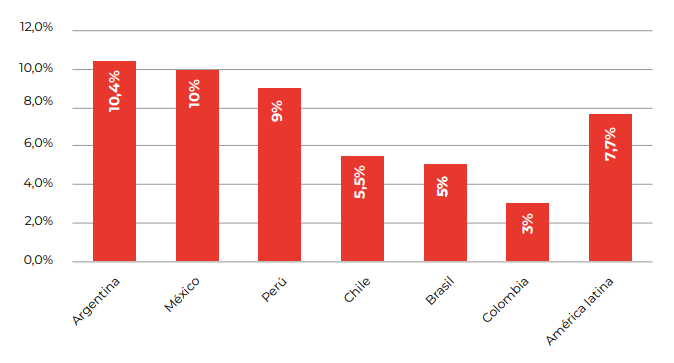
\includegraphics[width=0.8\textwidth]{gastotecnologia.png}
    \caption{Gasto en tecnologías de la información - América Latina. Fuente: \cite{ArticleRef255142}}
    \label{fig:gastos}
\end{figure}

\subsection{Desafío técnico desde la perspectiva de telecomunicaciones}

Desde la perspectiva de la ingeniería de telecomunicaciones, el problema central radica en la necesidad de desarrollar un sistema distribuido que permita el procesamiento automatizado de imágenes capturadas por dispositivos móviles para la determinación precisa de las dimensiones de paquetes. Este desafío implica la integración eficiente y confiable de múltiples componentes tecnológicos.

Actualmente, las telecomunicaciones facilitan la captura y el almacenamiento de información, como fotografías y ubicaciones GPS, que pueden contribuir al seguimiento en tiempo real de los procesos logísticos. No obstante, el avance tecnológico permite ir más allá del simple almacenamiento de datos, habilitando el procesamiento inteligente de la información para extraer datos adicionales que generen ahorros significativos en horas-hombre y mejoren sustancialmente la eficiencia operativa.

El desafío específico consiste en desarrollar una fuente confiable para la determinación automatizada de las medidas de los paquetes, que permita optimizar tanto las rutas de distribución como la carga asignada a cada motorizado durante los procesos de recojo y entrega. Esta solución debe aprovechar las capacidades de procesamiento en la nube para realizar análisis complejos de imágenes sin requerir dispositivos móviles con especificaciones premium, garantizando así la escalabilidad y accesibilidad del sistema.

\subsection{Características específicas del problema}

Desde la perspectiva de la ingeniería de telecomunicaciones, el problema central radica en la necesidad de desarrollar un sistema distribuido que permita el procesamiento automatizado de imágenes capturadas por dispositivos móviles, con el fin de determinar con precisión las dimensiones de los paquetes. Este desafío implica la integración eficiente y confiable de múltiples componentes tecnológicos.

Actualmente, las telecomunicaciones facilitan la captura y el almacenamiento de información, como fotografías y ubicaciones GPS, que pueden contribuir al seguimiento en tiempo real de los procesos logísticos. No obstante, el avance tecnológico permite ir más allá del simple almacenamiento de datos, habilitando el procesamiento inteligente de la información para extraer datos adicionales que generen ahorros significativos en horas-hombre y mejoren sustancialmente la eficiencia operativa.

El desafío específico consiste en desarrollar una fuente confiable para la determinación automatizada de las medidas de los paquetes, que permita optimizar tanto las rutas de distribución como la carga asignada a cada motorizado durante los procesos de recojo y entrega. Esta solución debe aprovechar las capacidades de procesamiento en la nube para realizar análisis complejos de imágenes sin requerir dispositivos móviles con especificaciones premium, garantizando así la escalabilidad y accesibilidad del sistema.
% ------------------------------------------------------------------
\section{Importancia del problema y su solución}
% ------------------------------------------------------------------

\subsection{Perspectiva técnica}

Resolver este problema es clave debido al uso de tecnologías emergentes que están transformando las telecomunicaciones y la computación distribuida. El procesamiento en la nube ha madurado lo suficiente como para realizar análisis complejos de imágenes sin necesidad de ejecución local en los dispositivos. Esto democratiza el acceso a capacidades avanzadas de procesamiento, permitiendo que empresas con recursos limitados accedan a soluciones sofisticadas sin requerir infraestructuras costosas.

Los algoritmos de visión por computadora en entornos de nube distribuida escalan dinámicamente el procesamiento, optimizando tanto el rendimiento como los costos. La integración del Internet de las Cosas (IoT) con telecomunicaciones avanzadas habilita aplicaciones inteligentes capaces de procesar datos en tiempo real y proporcionar retroalimentación inmediata. Esta convergencia resulta vital en la transformación digital de diversos sectores económicos, donde la capacidad de analizar grandes volúmenes de datos automatizados representa una ventaja competitiva \cite{RedaccinTLW2024,Jurez2023}.

\subsection{Perspectiva económica y financiera}

La automatización en la medición de paquetes contribuye directamente a mejorar la rentabilidad y la competitividad en los procesos logísticos, al generar ahorros significativos y optimizar el uso de recursos de transporte. El procesamiento en la nube permite reducir la inversión en dispositivos de alto costo, facilitando el acceso a tecnologías avanzadas para pequeñas y medianas empresas (pymes). Asimismo, elimina la necesidad de infraestructura local y personal técnico especializado, transformando los costos fijos en gastos operacionales escalables \cite{Krysiska2024}.

La optimización de rutas y la maximización de la carga útil permiten reducir el consumo de combustible y los tiempos operativos, lo que se traduce en un aumento de la productividad y una mejora en los márgenes de rentabilidad.

\begin{figure}[H]
    \centering
    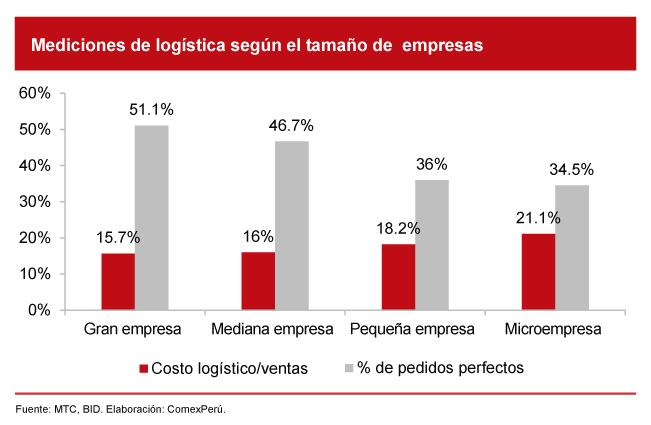
\includegraphics[width=0.8\textwidth]{gastoporempresa.png}
    \caption{Gasto en tecnologías de la información - América Latina. Fuente: \cite{ArticleRef255141}}
    \label{fig:gastos_tecnologia}
\end{figure}

\subsection{Perspectiva social y cultural}

Socialmente, la solución propuesta contribuye a mejorar la calidad de vida tanto de los trabajadores logísticos como de los usuarios finales. La automatización de tareas repetitivas permite redirigir los recursos humanos hacia actividades de mayor valor agregado, lo que favorece la satisfacción laboral y el desarrollo profesional.

La mayor precisión y confiabilidad en los procesos de entrega fortalece la confianza en los servicios digitales, facilitando el acceso oportuno a bienes, especialmente en poblaciones que dependen del \textit{delivery} como canal principal de abastecimiento. Además, la democratización de tecnologías avanzadas permite que las pequeñas y medianas empresas compitan en igualdad de condiciones con grandes corporaciones, fomentando la diversidad empresarial, la innovación, el empleo técnico especializado y el desarrollo local en sectores vinculados a tecnologías emergentes.

\subsection{Perspectiva ambiental y de sostenibilidad}
Abordar este problema es clave para reducir emisiones de gases de efecto invernadero y usar recursos energéticos eficientemente. La optimización de rutas, basada en medidas precisas de paquetes, permite planificar trayectos más cortos, disminuyendo consumo de combustible y emisiones de CO\textsubscript{2}.

La eficiencia en recojo y entrega, junto con rutas óptimas y verificación automatizada, hace las operaciones más cortas y seguras, minimizando el impacto ambiental y eliminando viajes innecesarios \cite{WebRef132362}.

Los ahorros energéticos incluyen también la reducción del trabajo manual y procesos administrativos repetitivos, optimizando recursos y contribuyendo a la sostenibilidad empresarial y sectorial.

\subsection{Perspectiva legal y reglamentaria}
\subsubsection{Cumplimiento de normativas de protección de datos}

En Perú, la medición automatizada de paquetes con IoT debe cumplir la Ley N.º 29733, que exige consentimiento previo, finalidad clara, calidad y seguridad en el tratamiento de datos \cite{EditoraPer2973}.
La solución debe proteger información sensible de remitentes, destinatarios, vehículos, empleados y clientes. Dado el gran volumen y flujo constante de datos, se requieren sólidas medidas de seguridad para garantizar el cumplimiento ético y legal.

\subsubsection{Estándares de calidad en servicios logísticos}
La logística demanda precisión, confiabilidad y transparencia. La automatización mediante sensores \textit{IoT} y algoritmos de \textit{Machine Learning} permite optimizar inventarios y rutas, proporcionando datos objetivos y verificables. El monitoreo continuo genera alertas tempranas ante anomalías, fortaleciendo el control de calidad y la conformidad normativa. La trazabilidad mejora la visibilidad en tiempo real, cumpliendo con las expectativas comerciales y las responsabilidades empresariales \cite{ArticleRef255132, ArticleRef255131}.

\subsubsection{Regulaciones de telecomunicaciones e \textit{IoT}}
Las normativas garantizan seguridad, interoperabilidad y conectividad. La Estrategia Nacional de IA en Perú impulsa el desarrollo de infraestructura digital y el despliegue de redes 5G, facilitando la adopción masiva de \textit{IoT}. La Red Dorsal Nacional de Fibra Óptica, con más de 13{,}500 km operativos, permite la conexión de dispositivos a gran escala. Además, el procesamiento distribuido mediante el Centro Nacional de Computación de Alto Rendimiento y los centros de datos en la nube fortalecen el \textit{edge computing} y mejoran el desempeño de aplicaciones logísticas inteligentes.

\subsubsection{Marco legal para la inteligencia artificial}
Se busca integrar la inteligencia artificial en los procesos empresariales mediante sistemas \textit{IoT} para realizar análisis en tiempo real, utilizando algoritmos capaces de detectar riesgos o anomalías. La gestión de \textit{Big Data} con sensores \textit{IoT} permite tomar decisiones estratégicas, respaldadas por políticas que fomentan el desarrollo de talento en computación paralela y procesamiento de señales. Asimismo, se promueve el desarrollo de aplicaciones móviles logísticas, aprovechando la alta penetración del internet móvil y los \textit{smartphones} para optimizar las entregas y monitorear las cargas en tiempo real \cite{ArticleRef255131}.


\subsection{Perspectiva ética}
\subsubsection{Responsabilidad Social y Laboral}

La automatización en la medición plantea un dilema ético entre la eficiencia y el empleo. Esta investigación propone un enfoque de complementariedad tecnológica, en el cual la automatización potencia las habilidades humanas en lugar de generar desplazamiento laboral. Es necesario diseñar interfaces que faciliten la reconversión profesional hacia tareas de mayor valor, como el análisis, la gestión de excepciones y la supervisión. Asimismo, se requieren programas de capacitación que permitan a los trabajadores adaptarse a nuevos roles, asegurando que la tecnología promueva el desarrollo humano sin generar exclusión social en los sectores logísticos.
\subsubsection{Equidad Digital y Democratización Tecnológica}
El diseño ético debe contribuir al cierre de brechas digitales, evitando que el avance tecnológico incremente las desigualdades entre empresas. Para ello, se requieren arquitecturas escalables, interfaces intuitivas y modelos de precios accesibles que favorezcan la adopción tecnológica por parte de pequeñas y medianas empresas. Asimismo, es fundamental considerar las diferencias en infraestructura regional, diseñando soluciones que funcionen adecuadamente tanto en zonas con buena conectividad como en aquellas que presentan limitaciones.
\subsubsection{Sostenibilidad Ambiental y Responsabilidad Climática}
La ética tecnológica incluye la evaluación de la huella de carbono generada por el procesamiento en la nube frente a los beneficios derivados de la optimización logística. Aunque la nube ofrece escalabilidad, su consumo energético debe ser balanceado con la reducción de emisiones lograda mediante un mejor aprovechamiento de espacios y la disminución de desplazamientos físicos. Es fundamental seleccionar proveedores comprometidos con el uso de energías renovables y desarrollar algoritmos eficientes que minimicen el consumo de recursos sin comprometer la precisión de los resultados.
\subsubsection{Privacidad de Datos y Soberanía Informacional}
El manejo ético de datos va más allá del cumplimiento legal, al enfocarse en la protección de información sensible relacionada con operaciones comerciales y logísticas. Es fundamental aplicar el principio de \textit{privacy by design}, incorporando mecanismos de anonimización, \textit{end-to-end encryption} y políticas estrictas de retención que limiten el almacenamiento únicamente al tiempo necesario.
\subsubsection{Responsabilidad y Rendición de Cuentas}
Es vital establecer mecanismos claros para gestionar errores, compensar daños económicos y permitir apelaciones frente a decisiones automatizadas. Asimismo, deben realizarse evaluaciones periódicas del impacto social, económico y ambiental, incorporando retroalimentación continua para maximizar los beneficios y mitigar los efectos negativos.

Esta visión ética integral garantiza que la tecnología respete los valores humanos y contribuya al desarrollo sostenible en el ámbito logístico, estableciendo un ejemplo responsable para futuras innovaciones.


% ------------------------------------------------------------------
\section{Impactos previstos y beneficiarios}
% ------------------------------------------------------------------

\subsection{Impactos operacionales}

La implementación de la solución propuesta tendrá impactos operacionales significativos, mejorando la eficiencia de los procesos logísticos mediante tecnologías \textit{IoT}, inteligencia artificial y visión artificial. Estas permiten recopilar, transmitir y analizar datos en tiempo real, automatizando tareas clave.

\subsubsection{Reducción de tiempos de procesamiento}

La medición automatizada de paquetes elimina procesos manuales, reduciendo el tiempo requerido para registrar, verificar y procesar solicitudes. Gracias al uso de tecnologías \textit{IoT} y al procesamiento masivo de datos, se agiliza la toma de decisiones y la selección de servicios adecuados, mejorando la experiencia del usuario \cite{RedaccinTLW2024, Sun2024, Wang2012}.

\subsubsection{Optimización de rutas de entrega}

Con datos precisos sobre las dimensiones de los paquetes, los sistemas pueden planificar rutas más eficientes considerando la capacidad de carga, el tiempo y la distancia. El uso de algoritmos de ruteo inteligente y planificación asistida por \textit{IA} permite reducir costos, tiempos y emisiones, contribuyendo además al desarrollo sostenible \cite{WebRef132365}.

\subsubsection{Precisión en estimaciones de capacidad}

La información confiable sobre los paquetes permite ajustar de manera más precisa la carga por vehículo, evitando excesos. El análisis de datos históricos y predictivos posibilita una logística anticipada, apoyada en componentes analíticos que procesan grandes volúmenes de información \textit{IoT} para mejorar la planificación operativa \cite{Alharbi2023, WebRef132362}.

\subsubsection{Automatización de verificaciones y trazabilidad}

La automatización proporciona evidencia visual y documental confiable en cada transacción, mejorando la seguridad y la resolución de disputas. Sensores, cámaras y dispositivos de rastreo permiten la supervisión y verificación en tiempo real a lo largo de toda la cadena logística \cite{RedaccinTLW2024}.

\subsubsection{Detección de anomalías}

El análisis en tiempo real permite identificar desvíos o condiciones anómalas en el transporte, activando alertas preventivas que fortalecen la seguridad y la confiabilidad del servicio \cite{RedaccinTLW2024}. En conjunto, estos impactos representan una transformación operativa integral, orientada a una mayor precisión, automatización y capacidad de respuesta en las operaciones logísticas.

\subsection{Impactos tecnológicos}

La implementación de esta solución tendrá un impacto tecnológico significativo en el ámbito de las telecomunicaciones y las tecnologías \textit{IoT}, estableciendo nuevos paradigmas en el procesamiento de imágenes aplicadas a la logística y demostrando el potencial de las arquitecturas distribuidas en la nube.
\subsubsection{Procesamiento distribuido para análisis de imágenes}

Utilizando modelos de lenguaje multimodal (\textit{LLMs}) especializados en análisis visual-semántico, la nube manejará grandes volúmenes de datos visuales generados por dispositivos \textit{IoT}. Esta arquitectura escalable facilitará el análisis en tiempo real de millones de imágenes para medir automáticamente dimensiones de paquetes. Esto reducirá costos al reemplazar mediciones manuales, mejorará la precisión y permitirá el monitoreo remoto continuo, optimizando la logística automatizada.

\subsubsection{Integración con telecomunicaciones y aplicaciones móviles}

La propuesta combina procesamiento intensivo con interfaces móviles accesibles, aprovechando redes 4G/5G para transmitir imágenes en alta resolución de manera eficiente. La arquitectura soporta miles de dispositivos simultáneamente, garantizando escalabilidad para grandes implementaciones empresariales. Además, se conecta con infraestructura existente para reducir la latencia y mejorar los tiempos de respuesta y la experiencia del usuario.

Así, se habilita el análisis de grandes volúmenes de datos visuales, sentando las bases para soluciones \textit{Big Data} que cumplan con precisión, rapidez y confiabilidad en la medición automatizada de paquetes.

\subsubsection{Innovación en aplicaciones móviles para logística}

Se desarrollarán aplicaciones fáciles de usar para que usuarios no técnicos capturen dimensiones complejas mediante fotografías. La aplicación permitirá el monitoreo en tiempo real y el seguimiento preciso. Integrada con bases \textit{NoSQL} y microservicios, la solución asegura escalabilidad y despliegue eficiente en la nube, aprovechando tecnologías \textit{BaaS} para optimizar el rendimiento. La automatización transformará los centros de distribución, reduciendo tiempos y mejorando la precisión, además de facilitar la comunicación directa entre operadores y sistemas de gestión.

\subsubsection{Impacto transformacional en logística}

Estos avances promoverán una transformación profunda, mejorando la eficiencia, precisión y transparencia. La solución habilitará sistemas inteligentes adaptables a las demandas del mercado, ofreciendo mayor visibilidad y control en la medición y clasificación de paquetes. Su adopción facilitará decisiones en tiempo real, optimizando recursos e inventarios, y sentará precedentes para aplicar soluciones similares en otros sectores que requieran procesamiento automatizado de datos visuales y mediciones precisas con tecnologías móviles y en la nube.


\subsection{Impactos económicos}

Los impactos económicos se reflejan desde la productividad individual hasta la competitividad sectorial, aprovechando el procesamiento de imágenes con \textit{IA} en la nube para optimizar las entregas urbanas.

\subsubsection{Maximización de productividad de motorizados}

Se optimiza la capacidad de transporte y se reducen tiempos improductivos mediante ruteo inteligente con algoritmos que asignan rutas más cortas y eficientes, disminuyendo tiempos y consumo de combustible, lo que permite realizar más entregas por viaje \cite{WebRef132362}. El monitoreo en tiempo real facilita decisiones rápidas y reduce intentos fallidos, mejorando la experiencia del cliente.

\subsubsection{Reducción de costos operacionales}

Incluye ahorro en combustible, tiempo de personal, comunicación y administración. El ruteo optimizado minimiza kilómetros recorridos y desgaste vehicular, generando hasta un 15\% de ahorro. La automatización reduce costos de mano de obra y mantenimiento. El monitoreo previene pérdidas y daños al activar alertas ante anomalías. La infraestructura en la nube asegura procesamiento eficiente y escalable, evitando inversiones locales costosas \cite{RedaccinTLW2024}.

\subsubsection{Mejora en la rentabilidad empresarial}

La combinación de menores costos y mayores ingresos permite procesar más pedidos con la misma infraestructura, aumentando la rentabilidad y competitividad. Se estima una reducción de costos logísticos superior al 30\% y una mejora operativa de hasta el 40\%. La satisfacción del cliente se incrementa gracias a la visibilidad y las entregas puntuales, fomentando la lealtad y la repetición de compra. El análisis de datos fortalece las decisiones estratégicas en demanda, inventarios y gestión de riesgos.

\subsubsection{Generación de nuevo valor agregado}

Se crean servicios diferenciados mediante el uso de datos detallados para modelos de estimación de precios precisos. El \textit{Quick Commerce} se potencia con entregas en menos de 90 minutos, mejorando la eficiencia en la última milla. El análisis en tiempo real habilita la personalización y la transparencia. La optimización de rutas favorece la sostenibilidad, reduciendo emisiones y reforzando la imagen ecológica como una ventaja competitiva clave \cite{WebRef132364}.


\subsection{Beneficiarios directos}

\subsubsection{Empresas de delivery y logística}

Son los principales beneficiarios, mejorando la eficiencia y la rentabilidad gracias al procesamiento de imágenes con \textit{IA} en la nube. La optimización del ruteo reduce kilómetros recorridos y consumo de combustible, generando hasta un 15\% de ahorro en costos y desgaste vehicular. La infraestructura en la nube proporciona recursos escalables, evitando inversiones locales costosas. La rentabilidad mejora al gestionar más pedidos con los mismos recursos, reduciendo los costos logísticos en más del 30\% y aumentando la eficiencia hasta en un 40\%. Además, la logística verde contribuye a reducir emisiones y fortalecer la imagen de marca.

\subsubsection{Motorizados y personal operativo}

Mejoran su productividad y condiciones laborales mediante rutas optimizadas que permiten realizar más entregas en menos tiempo. La visión artificial facilita la identificación del tamaño de los paquetes, optimizando la carga y agilizando la operación. Esto reduce el estrés y la incertidumbre, mejorando los ingresos y las condiciones laborales. El monitoreo en tiempo real incrementa la seguridad al alertar sobre riesgos y desvíos.

\subsubsection{Clientes emisores de paquetes}

Experimentan mayor fiabilidad y transparencia gracias a rutas inteligentes que optimizan las entregas y el recojo. La captura fotográfica automatiza la medición del paquete, acelerando el proceso. La inspección automatizada mediante visión artificial garantiza calidad y confianza. La trazabilidad en tiempo real, combinando tecnologías \textit{IoT} e imágenes en la nube, permite rastrear los paquetes en cualquier momento \cite{WebRef132361}.

\subsubsection{Destinatarios de entregas}

Reciben un servicio más rápido y predecible, cumpliendo con los estándares de \textit{quick commerce} en menos de 90 minutos. La comunicación en tiempo real ofrece seguimiento del paquete y contacto directo con el repartidor, reduciendo los intentos fallidos. La experiencia mejora gracias a la rapidez, precisión y transparencia, fomentando la lealtad. El monitoreo ambiental previene daños, asegurando la llegada en óptimas condiciones \cite{WebRef132362}.


\subsection{Beneficiarios indirectos}

\subsubsection{Para el sector de telecomunicaciones}

Este sector verá un aumento en la demanda de servicios especializados y mejoras en infraestructura. La solución incrementará la necesidad de conectividad fija y móvil de alta velocidad, impulsando la adopción de tecnologías 4G y 5G para procesar grandes volúmenes de datos en tiempo real. La arquitectura en la nube motivará inversiones en servicios como \textit{IaaS}, \textit{PaaS} y \textit{FaaS}, además de optimizar redes y detectar anomalías, estimulando inversiones en centros de datos locales.

\subsubsection{Para la industria de desarrollo de software}

Se generarán nuevas oportunidades y mayor demanda de talento especializado en aplicaciones móviles, bases \textit{NoSQL}, microservicios y despliegue en la nube. La solución promoverá mejores prácticas para aplicaciones \textit{IoT} integradas con la nube, fomentará la investigación y el desarrollo local, y fortalecerá la colaboración academia-industria, alineándose con la Estrategia Nacional de Inteligencia Artificial (ENIA) del Perú \cite{ArticleRef255132}.

\subsubsection{Para el medio ambiente y la sociedad}

La optimización de rutas reducirá las emisiones de CO\textsubscript{2} y el consumo de combustible, contribuyendo a un entorno urbano más saludable \cite{WebRef13249}. Menor congestión vehicular y menos viajes innecesarios mejorarán la movilidad en Lima, incentivando el uso de vehículos eléctricos y bicicletas para la última milla. Estos beneficios respaldan la \textit{Logística 5.0}, que integra innovación tecnológica con sostenibilidad ambiental \cite{WebRef132362}.

\subsubsection{Para el ecosistema de innovación tecnológica}

La solución fortalecerá la innovación al demostrar cómo las tecnologías emergentes pueden resolver problemas reales. Actuará como catalizador para la madurez tecnológica y la formación en inteligencia artificial, alineándose con la ENIA, y fomentará la colaboración entre academia, industria y emprendedores. El proyecto puede mejorar la posición del Perú en los índices globales de \textit{IA} y servir como modelo para futuras implementaciones públicas y privadas \cite{ArticleRef255132}.

\vspace{1em}

La implementación de sistemas automatizados de medición de paquetes mediante tecnologías \textit{IoT} y procesamiento de imágenes en la nube representa un avance significativo hacia la logística inteligente del futuro. Los impactos multidimensionales de esta solución demuestran el potencial transformador de la convergencia tecnológica en telecomunicaciones, beneficiando directamente a empresas de \textit{delivery}, motorizados y usuarios finales, mientras fortalece el ecosistema de innovación tecnológica nacional. Este proyecto establece un precedente para futuras aplicaciones de \textit{IoT} en sectores críticos y contribuye al desarrollo de una infraestructura digital robusta que posiciona al país en la vanguardia de la transformación logística global.
